\chapter{Trajectory Tracking Error Dynamics}

The underwater robot system is a strongly coupled nonlinear system. Traditionally, the underwater robot dynamics is lineazied about constant states with specific values. For instance, in~\cite{F2011} (pp.174), low-speed application is assumed for neutrally buoyant submersible. Thus, the nonlinear Coriolis, centripetal, damping, restoring and buoyancy forces and moments can be linearized about $\vec{\upsilon}=\vec{0}$ and $\phi=\theta=0$. The linearized manoeuvring model (\cite{F2011}, pp.131)  for marine craft is based on the assumption of constant cruise speed $U$. Also, the nonlinear damping is approximated by a linear damping matrix. 

In this  work, we present a path-based linearization method for the error dynamics between robot's real states and the path-determined states. Our method is in essence also linearization about constant states. Nevertheless, our linearization is based on all dynamic (velocities) and kinematic (position and Euler angles) states except for the yaw angle $\psi$ instead several of them. Therefore, we bring nearly the full information of the trajectory into the linearized model. Furthermore, we do not require explicit values for these states. In other words, our linearized model is a function of the states. For a specific trim trajectory, we evaluate the function with explicit values from the trajectory specifications. The state variables of underwater robots can be divided into two groups, i.e., kinematic states and dynamic states. Dynamic states include three linear and three angular velocities represented in the robot frame $\lbrace b \rbrace$:
\begin{align}
\vec{x}_{dyn}=\vec{\upsilon}=
\begin{pmatrix}
\vec{v}\\ \vec{\omega}
\end{pmatrix}=
\begin{pmatrix}
u\\v\\w\\p\\q\\r
\end{pmatrix}
\in 
\mathbb{R}^{6}.
\end{align}
Kinematic states consist of the position and orientation of the underwater robot in the inertial world frame $\lbrace i \rbrace$:
\begin{align}
\vec{x}_{kin}=\vec{\eta}=
\begin{pmatrix}
\vec{p} \\ \vec{\lambda}
\end{pmatrix}=
\begin{pmatrix}
x \\ y \\ z \\ \phi \\ \theta\\ \psi
\end{pmatrix}
\in 
\mathbb{R}^{6}.
\end{align}
The whole states are defined as:
\begin{align}
\vec{x}=
\begin{pmatrix}
\vec{x}_{dyn}\\ \vec{x}_{kin}
\end{pmatrix}
\in 
\mathbb{R}^{12}.
\end{align}
The state space representation $\mathcal{P}$ of nonlinear underwater robot system can be written in the following form:
\begin{align}
\mathcal{P}
\coloneqq
\dfrac{d}{dt}
\begin{pmatrix}
\vec{x}_{dyn} \\
\vec{x}_{kin}
\end{pmatrix}=
\begin{pmatrix}
\mathfrak{F}_{dyn}(\vec{x}_{dyn},\vec{x}_{kin})\\
\mathfrak{F}_{kin}(\vec{x}_{dyn},\vec{x}_{kin})
\end{pmatrix}+
\begin{pmatrix}
\mathfrak{B}(\vec{x}_{dyn})\mathfrak{H}(\vec{x}_{dyn},\vec{u})\\0
\end{pmatrix}
\end{align}
Now, we want to reformulate the standard underwater robot equations of motion
\begin{align}
\emph{\textbf{M}}\dot{\vec{\upsilon}}+\emph{\textbf{C}}(\vec{\upsilon})\vec{\upsilon}+\emph{\textbf{D}}(\vec{\upsilon})\vec{\upsilon}+\vec{g}(\vec{\eta})=\vec{\tau}
\label{EQ:Dy}
\end{align}
into the aforementioned form.


More precisely, we want to identify all the terms in the following equations from the robot dynamics and kinematics. 
\begin{empheq}[left=\mathcal{P}:\empheqlbrace]{align}
& \dfrac{d}{dt}\vec{v}=\mathfrak{F}_{\vec{v}}(\vec{v},\vec{\omega})+\mathfrak{F}_{\vec{v}}^{\lambda}(\Pi_{i}\vec{\lambda})+\mathfrak{B}_{\vec{v}}(\vec{v},\vec{\omega})\mathfrak{H}(\vec{v},\vec{u}) \label{EQ:P1}\\
&\dfrac{d}{dt}\vec{\omega}=\mathfrak{F}_{\vec{\omega}}(\vec{v},\vec{\omega})+\mathfrak{F}_{\omega}^{\lambda}(\Pi_{i}\vec{\lambda})+\mathfrak{B}_{\omega}(\vec{v},\vec{\omega})\mathfrak{H}(\vec{v},\vec{u}) \label{EQ:P2} \\
& \dfrac{d}{dt}\vec{p}=\emph{\textbf{R}}(\lambda)\vec{v} \label{EQ:P3} \\
&\dfrac{d}{dt}\vec{\lambda}=\emph{\textbf{Q}}(\Pi_{i}\vec{\lambda})\vec{\omega}\label{EQ:P4}.
\end{empheq}
where $\vec{\lambda}$ represents the Euler angles ($\phi$, $\theta$, $\psi$) and $\Pi_{i}\vec{\lambda}=(\phi, \theta)^{T}$ denotes the two kinematic states appearing in the underwater robot dynamics since the restoring term $\vec{g}(\eta)$ includes the two angles. $\emph{\textbf{R}}(\lambda)$ is the linear velocity transformation matrix and $\emph{\textbf{Q}}(\Pi_{i}\vec{\lambda})$ is the angular velocity transformation matrix. 
The dynamic equation \ref{EQ:Dy} can be rewritten as 
\begin{align}
\dot{\vec{\upsilon}}=-\emph{\textbf{M}}^{-1}\emph{\textbf{C}}(\vec{\upsilon})\vec{\upsilon}-\emph{\textbf{M}}^{-1}\emph{\textbf{D}}(\vec{\upsilon})\vec{\upsilon}-\emph{\textbf{M}}^{-1}\emph{\textbf{g}}(\vec{\eta})+\emph{\textbf{M}}^{-1}\tau.
\end{align}
Note that the inertia matrix $\emph{\textbf{M}}$ is the sum of the rigid body inertia matrix $\emph{\textbf{M}}_{RB}$ and the added mass inertia matrix $\emph{\textbf{M}}_{A}$, the Coriolis matrix $\emph{\textbf{C}}(\vec{\upsilon})$ includes the rigid body Coriolis matrix $\emph{\textbf{C}}_{RB}(\vec{\upsilon})$ and the added mass Coriolis matrix $\emph{\textbf{C}}_{A}$. 
We assign the first three rows of the rigid body added mass $\emph{\textbf{C}}_{RB}(\vec{v},\vec{\omega})$ matrix into sub-matrices $\emph{\textbf{C}}_{RB,\vec{v}}(\vec{v},\vec{\omega})$ and the last three rows into sub-matrices $\emph{\textbf{C}}_{RB,\vec{\omega}}(\vec{v},\vec{\omega})$:
\begin{align}
\emph{\textbf{C}}_{RB,\vec{v}}(\vec{v},\vec{\omega})=
\begin{pmatrix}
0&0&0&m(y_{g}q+z_{g}r)&-m(x_{g}q-w)&-m(x_{g}r+v)\\
0&0&0&-m(y_{g}p+w)&m(z_{g}r+x_{g}p)&-m(y_{g}r-u)\\
0&0&0&-m(z_{g}p-v)&-m(z_{g}q+u)&m(x_{g}p+y_{g}q)\\
\end{pmatrix} \label{EQ:CoriolisRigidBodyV}
\end{align}
and
\begin{gather}\label{EQ:CoriolisRigidBodyW}
\emph{\textbf{C}}_{RB,\vec{\omega}}(\vec{v},\vec{\omega})=
\left(
\begin{matrix} -m(y_{g}+z_{g}r)&m(y_{g}p+w)&m(z_{g}p-v)\\
m(x_{g}q-w)&-m(z_{g}r+x_{g}p)&m(z_{g}q+u)\\
m(x_{g}r+v)&m(y_{g}r-u)&-m(x_{g}p+y_{g}q)
\end{matrix}
\right.
 \nonumber\\
\qquad \qquad\left. \begin{matrix} 
0 & -I_{yz}q-I_{xz}p+I_{z}r & I_{yz}r+I_{xy}p-I_{y}q \\
I_{yz}q+I_{xz}p-I_{z}r &0& -I_{xz}r-I_{xy}q+I_{x}p \\
-I_{yz}r-I_{xy}p+I_{y}q&I_{xz}r+I_{xy}q-I_{x}p &0  \end{matrix}
\right).
%\end{equation}
\end{gather}
Similarly, the added mass Coriolis matrix can be also divided into two parts $\emph{\textbf{C}}_{A,\vec{v}}(\vec{v},\vec{\omega})$ and $\emph{\textbf{C}}_{A,\vec{\omega}}(\vec{v},\vec{\omega})$, where
\begin{align}
\emph{\textbf{C}}_{A,\vec{v}}(\vec{v},\vec{\omega})=
\begin{pmatrix}
0&0&0&0&-Z_{\dot{w}}w&Y_{\dot{v}}v\\
0&0&0&Z_{\dot{w}}w&0&-X_{\dot{u}}u\\
0&0&0&-Y_{\dot{v}}v&X_{\dot{u}}u&0
\end{pmatrix}
\end{align} 
and
\begin{align}
\emph{\textbf{C}}_{A,\vec{\omega}}(\vec{v},\vec{\omega})=
\begin{pmatrix}
0&-Z_{\dot{w}}w&Y_{\dot{v}}v&0&-N_{\dot{r}}\dot{r}&M_{\dot{q}}q\\
Z_{\dot{w}}w&0&-X_{\dot{u}}u&N_{\dot{r}}r&0&-K_{\dot{p}}p\\
-Y_{\dot{v}}v&X_{\dot{u}}u&0&-M_{\dot{q}}q&K_{\dot{p}}p&0
\end{pmatrix}.
\end{align}
For the drag matrix, we perform the same separation:
\begin{align}
\emph{\textbf{D}}_{\vec{v}}=
\begin{pmatrix}
-X_{u|u|}|u|&0&0&0&0&0\\
0&-Y_{v|v|}|v|&0&0&0&0\\
0&0&-Z_{w|w|}|w|&0&0&0\\
\end{pmatrix}
\end{align}
\begin{align}
\emph{\textbf{D}}_{\vec{\omega}}=
\begin{pmatrix}
0&0&0&-K_{p|p|}|p|\\
0&0&0&0&-M_{q|q|}|q|\\
0&0&0&0&0&-N_{r|r|}|r|\\
\end{pmatrix}.
\end{align}
The restoring term 
\begin{align}
\vec{g}(\vec{\eta})=
\begin{pmatrix}
(W-B)\sin(\theta)\\
-(W-B)\cos(\theta)\sin(\phi)\\
-(W-B)\cos(\theta)\cos(\phi)\\
-(y_{g}W-y_{b}B)\cos(\theta)\cos(\phi)+(z_{g}W-z_{b}B)\cos(\theta)\sin(\phi)\\
(z_{g}W-z_{b}B)\sin(\theta)+(x_{g}W-x_{b}B)\cos(\theta)\cos(\phi)\\
-(x_{g}W-x_{b}B)\sin(\theta)\cos(\phi)-(y_{g}W-y_{b}B)\sin(\theta)
\end{pmatrix} \label{EQ:Restoring}
\end{align}
can also be separated into the following two terms
\begin{align}
\vec{g}_{\vec{v}}(\vec{\eta})=
\begin{pmatrix}
(W-B)\sin(\theta)\\
-(W-B)\cos(\theta)\sin(\phi)\\
-(W-B)\cos(\theta)\cos(\phi)
\end{pmatrix} \label{EQ:RestoringV}
\end{align}
\begin{align}
\vec{g}_{\vec{\omega}}(\vec{\eta})=
\begin{pmatrix}
-(y_{g}W-y_{b}B)\cos(\theta)\cos(\phi)+(z_{g}W-z_{b}B)\cos(\theta)\sin(\phi)\\
(z_{g}W-z_{b}B)\sin(\theta)+(x_{g}W-x_{b}B)\cos(\theta)\cos(\phi)\\
-(x_{g}W-x_{b}B)\sin(\theta)\cos(\phi)-(y_{g}W-y_{b}B)\sin(\theta)
\end{pmatrix},\label{EQ:RestoringW}
\end{align}
where $W$ is the total weight of the robot, and $B$ denotes the total buoyancy. $\vec{r}_{g}=(x_{g}, y_{g}, z_{g})^{T}$ is the center of gravity vector and $\vec{r}_{b}=(x_{b}, y_{b}, z_{b})^{T}$ is the center of buoyancy vector.
After reordering the Coriolis matrix, the damping matrix and the restoring matrix and comparing them with~\ref{EQ:P1} and~\ref{EQ:P2}, we can obtain the following equations:
\begin{align}
\mathfrak{F}_{\vec{v}}(\vec{v},\vec{\omega})=
-\emph{\textbf{M}}^{-1}(\emph{\textbf{C}}_{RB,\vec{v}}+\emph{\textbf{C}}_{A,\vec{v}}+\emph{\textbf{D}}_{\vec{v}})
\end{align}
\begin{align}
\mathfrak{F}_{\vec{\omega}}(\vec{v},\vec{\omega})=
-\emph{\textbf{M}}^{-1}(\emph{\textbf{C}}_{RB,\vec{\omega}}+\emph{\textbf{C}}_{A,\vec{\omega}}+\emph{\textbf{D}}_{\vec{\omega}})
\end{align}
\begin{align}
\mathfrak{F}_{\vec{\omega}}^{\vec{\lambda}}(\Pi_{i}\vec{\lambda})=
-\emph{\textbf{M}}^{-1}\vec{g}_{\vec{\omega}}(\vec{\eta})
\end{align}
\begin{align}
\mathfrak{F}_{\vec{v}}^{\vec{\lambda}}(\Pi_{i}\vec{\lambda})=
-\emph{\textbf{M}}^{-1}\vec{g}_{\vec{v}}(\vec{\eta}).
\end{align}
Now, let us come to the input part, $\vec{u}$ is the control input generated by fins and thrusters. Suppose we have $n_{t}$ thrusters and $n_{f}$ fins, then it can be written as 
\begin{align}
\vec{u}=(u_{T,1}\cdots u_{T,n_{t}}~ \delta_{F,1} \cdots \delta_{F,n_{f}})^{T}\in \mathbb{R}^{(n_{t}+n_{f})\times 1}. 
\end{align}
For each actuator there is a corresponding input mapping vector and we can formulate the input matrix as $\emph{\textbf{B}}_{a}=(\emph{\textbf{B}}_{T,1} \cdots \emph{\textbf{B}}_{T,n_{t}}~\emph{\textbf{B}}_{F,1} \cdots \emph{\textbf{B}}_{F,n_{f}})\in \mathbb{R}^{6\times(n_{t}+n_{f})}$.
The first three rows of the matrix $\emph{\textbf{B}}_{a}$ are denoted by $\emph{\textbf{B}}_{a,f}\in \mathbb{R}^{3\times(n_{t}+n_{f})}$ and the last three rows of the matrix are represented by $\emph{\textbf{B}}_{a,m}\in \mathbb{R}^{3\times(n_{t}+n_{f})}$. The generalized force generated by the actuators can be represented as $\vec{\tau}=\emph{\textbf{B}}_{a}\vec{u}$. Separately written, $\vec{f}=\emph{\textbf{B}}_{a,f}\vec{u}$ and $\vec{m}=\emph{\textbf{B}}_{a,m}\vec{u}$, where $\vec{f}$ is the force vector along x-, y- and z- axes and $\vec{m}$ is the moment vector about x-, y- and z-axes of the body frame $\lbrace b \rbrace$.

Hence, for our modeling methods, 
\begin{align}
\mathfrak{B}_{\vec{v}}(\vec{v},\vec{\omega})\mathfrak{H}(\vec{v},\vec{u})=
\emph{\textbf{M}}^{-1}\emph{\textbf{B}}_{a,f}\vec{u},
\end{align}
\begin{align}
\mathfrak{B}_{\vec{\omega}}(\vec{v},\vec{\omega})\mathfrak{H}(\vec{v},\vec{u})=
\emph{\textbf{M}}^{-1}\emph{\textbf{B}}_{a,m}\vec{u}.
\end{align}

This finishes the transformation of the robot dynamics into standard state space form.
\section{Nonlinear Transformation and Error Dynamics}
Figure~\ref{FIG:FrameRelationship} shows the relationship between different frames, the $\lbrace i \rbrace$ denotes the inertial world frame, and $\emph{\textbf{R}}$ represents the coordinate transformation from $\lbrace i \rbrace$ to the real robot frame $\lbrace b \rbrace$. $\lbrace \mathcal{T} \rbrace$ denotes the Frenet-Serret frame along the trim trajectory, ideally the robot body frame $\lbrace b \rbrace$ should coincide with the the frame $\lbrace \mathcal{T} \rbrace$ for a perfect tracking, but it is not necessarily the case in reality. Thus, we use $\emph{\textbf{R}}_{E}$ to denote the transformation matrix from the body frame $\lbrace b \rbrace$ to the trim frame $\lbrace \mathcal{T} \rbrace$ and $\emph{\textbf{R}}_{\mathcal{T}}$ to denote the transformation matrix from the trim frame $\lbrace \mathcal{T} \rbrace$ to the inertial world frame $\lbrace i \rbrace$. Based on these definitions, we have the following relationship:
\begin{align}
\emph{\textbf{R}}_{E}=\emph{\textbf{R}}^{-1}_{\mathcal{T}}\emph{\textbf{R}}.
\end{align}     
\begin{figure}
\center
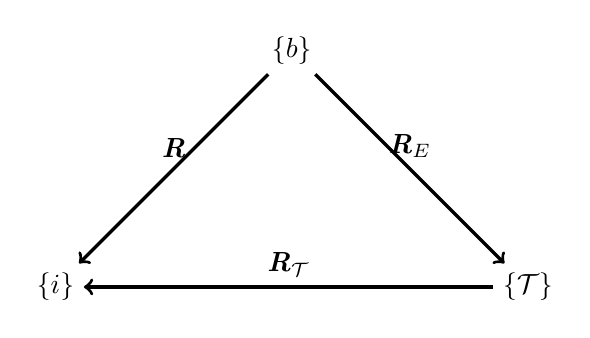
\begin{tikzpicture}
\node (A) at (0,0){$\lbrace i \rbrace$};
\node (B) at (3,3){$\lbrace b \rbrace$};
\node (C) at (6,0){$\lbrace \mathcal{T} \rbrace$};
\draw[->, very thick] (B) to
node[above] {$\emph{\textbf{R}}$} (A);
\draw[->, very thick] (C) to
node[above] {$\emph{\textbf{R}}_{\mathcal{T}}$} (A);
\draw[->, very thick] (B) to
node[above] {$\emph{\textbf{R}}_{E}$} (C);
\end{tikzpicture}
\caption{Frame relationship}	
\label{FIG:FrameRelationship}
\end{figure}
The desired states can be calculated from the predefined reference trim trajectories. Now we want to formulate the error dynamics. The velocities errors are defined intuitively as the difference between the desired velocity and the real velocity:
\begin{align}
\vec{v}_{E}=\vec{v}-\vec{v}_{\mathcal{T}}, \label{EQ:NLT1}
\end{align}
\begin{align}
\vec{\omega}_{E}=\vec{\omega}-\vec{\omega}_{\mathcal{T}}. \label{EQ:NLT2}
\end{align}
The position and orientation are defined in the inertial world frame $\lbrace i \rbrace$. We want to observe all the errors in the body frame $\lbrace b \rbrace$
\begin{align}
\vec{p}_{E}=\emph{\textbf{R}}^{-1}(\vec{p}-\vec{p}_{\mathcal{T}}) \label{EQ:NLT3}
\end{align}
\begin{align}
\vec{\lambda}_{E}=\emph{\textbf{Q}}^{-1}(\vec{\lambda}-\vec{\lambda}_{\mathcal{T}}) \label{EQ:NLT4}
\end{align}
Since the desired velocities $\vec{\upsilon}_{\mathcal{T}}$ and $\vec{\omega}_{\mathcal{T}}$ are constant along the trim trajectory, then we can obtain the following relationships for the derivative of velocity errors:
\begin{align}
\dfrac{d}{dt}\vec{v}_{E}=\dfrac{d}{dt}\vec{v}-\dfrac{d}{dt}\vec{v}_{\mathcal{T}}=\dfrac{d}{dt}\vec{v}
\end{align}
\begin{align}
\dfrac{d}{dt}\vec{\omega}_{E}=\dfrac{d}{dt}\vec{\omega}-\dfrac{d}{dt}\vec{\omega}_{\mathcal{T}}=\dfrac{d}{dt}\vec{\omega}.
\end{align}
In the following, we study the error kinematics.
We start from the nonlinear position transformation equation. 
\begin{align}
\vec{p}_{E}&=\emph{\textbf{R}}^{-1}(\vec{p}-\vec{p}_{\mathcal{T}}) \Rightarrow\nonumber \\
\vec{p}_{\mathcal{T}}&=\vec{p}-\emph{\textbf{R}}\vec{p}_{E}.
\end{align}
Taking derivative of both sides, we obtain 
\begin{align}
\dfrac{d}{dt}\vec{p}_{\mathcal{T}}=\dfrac{d}{dt}\vec{p}-(\dfrac{d}{dt}\emph{\textbf{R}})\vec{p}_{E}-\emph{\textbf{R}}(\dfrac{d}{dt}\vec{p}_{E}).
\end{align}
Since $\dfrac{d}{dt}\emph{\textbf{R}}(\vec{\lambda})=\emph{\textbf{R}}(\vec{\lambda})\emph{\textbf{S}}(\vec{\omega})$, we have the following equation:
\begin{align}
\dfrac{d}{dt}\vec{p}_{\mathcal{T}}=\dfrac{d}{dt}\vec{p}-\emph{\textbf{R}}\emph{\textbf{S}}(\vec{\omega})\vec{p}_{E}-\emph{\textbf{R}}(\dfrac{d}{dt}\vec{p}_{E}).
\end{align}
Reforming it, we get
\begin{align}
\emph{\textbf{R}}_{\mathcal{T}}\vec{v}_{\mathcal{T}}=\emph{\textbf{R}}\vec{v}-\emph{\textbf{R}}
\emph{\textbf{S}}(\vec{\omega})\vec{p}_{E}-\emph{\textbf{R}}\dfrac{d}{dt}\vec{p}_{E}.
\end{align}
Premultiplying both sides by $\emph{\textbf{R}}^{-1}$ and using $ \emph{\textbf{R}}_{E}^{-1}=\emph{\textbf{R}}^{-1}\emph{\textbf{R}}_{\mathcal{T}}$
\begin{align}
\dfrac{d}{dt}\vec{p}_{E}=\vec{v}-\emph{\textbf{R}}_{E}^{-1}\vec{v}_{\mathcal{T}}
-\emph{\textbf{S}}(\vec{\omega})\vec{p}_{E}
\end{align}
For the orientation error, we take the first derivative of the orientation transformation equation
\begin{align}
\vec{\lambda}_{E}&=\emph{\textbf{Q}}^{-1}(\vec{\lambda}-\vec{\lambda}_{\mathcal{T}}) \nonumber \\ \Rightarrow
\dfrac{d}{dt}\vec{\lambda}_{E}&=\emph{\textbf{Q}}^{-1}(\dfrac{d}{dt}\vec{\lambda}-\dfrac{d}{dt}\vec{\lambda}_{\mathcal{T}})+(\dfrac{d}{dt}\emph{\textbf{Q}}^{-1})(\vec{\lambda}-\vec{\lambda}_{\mathcal{T}}).
\end{align}
Since 
\begin{align}
\dfrac{d}{dt}\vec{\lambda}=\emph{\textbf{Q}}\vec{\omega}
\end{align}
and 
\begin{align}
\dfrac{d}{dt}\vec{\lambda}_{\mathcal{T}}=\emph{\textbf{Q}}_{\mathcal{T}}
\vec{\omega}_{\mathcal{T}},
\end{align}
we obtain 
\begin{align}
\dfrac{d}{dt}\vec{\lambda}_{E}=\emph{\textbf{Q}}^{-1}\emph{\textbf{Q}}\vec{\omega}
-\emph{\textbf{Q}}^{-1}\emph{\textbf{Q}}_{\mathcal{T}}
\vec{\omega}_{\mathcal{T}}
+(\dfrac{d}{dt}\emph{\textbf{Q}}^{-1})(\vec{\lambda}-\vec{\lambda}_{\mathcal{T}})\Rightarrow \nonumber \\
\dfrac{d}{dt}\vec{\lambda}_{E}=\vec{\omega}
-\emph{\textbf{Q}}^{-1}\emph{\textbf{Q}}_{\mathcal{T}}
\vec{\omega}_{\mathcal{T}}
+(\dfrac{d}{dt}\emph{\textbf{Q}}^{-1})\emph{\textbf{Q}}\vec{\lambda}_{E}
\end{align}

To sum up, the nonlinear error dynamic model $ \mathcal{P}_{E} $ for a given trim trajectory set is formulated as follows:
\begin{empheq}[left=\mathcal{P}_{E}:\empheqlbrace]{align}
&\dfrac{d}{dt}\vec{v}_{E}=\mathfrak{F}_{\vec{v}}(\vec{v},\vec{\omega})+\mathfrak{F}_{\vec{v}}^{\vec{\lambda}}(\Pi_{i}\vec{\lambda})+\mathfrak{B}_{\vec{v}}(\vec{v},\vec{\omega})\mathfrak{H}(\vec{v},\vec{u}) \\
&\dfrac{d}{dt}\vec{\omega}_{E}=\mathfrak{F}_{\vec{\omega}}(\vec{v},\vec{\omega})+\mathfrak{F}_{\vec{\omega}}^{\vec{\lambda}}(\Pi_{i}\vec{\lambda})+\mathfrak{B}_{\vec{\omega}}(\vec{v},\vec{\omega})\mathfrak{H}(\vec{v},\vec{u})\\
&\dfrac{d}{dt}\vec{p}_{E}=\vec{v}-\emph{\textbf{R}}_{E}^{-1}\vec{v}_{\mathcal{T}}
-\emph{\textbf{S}}(\vec{\omega}_{\mathcal{T}})\vec{p}_{E}\\
&\dfrac{d}{dt}\vec{\lambda}_{E}=\vec{\omega}
-\emph{\textbf{Q}}^{-1}\emph{\textbf{Q}}_{\mathcal{T}}
\vec{\omega}_{\mathcal{T}}
+(\dfrac{d}{dt}\emph{\textbf{Q}}^{-1})\emph{\textbf{Q}}\vec{\lambda}_{E}.
\end{empheq}
We define the the error dynamics input as
\begin{align}
\vec{u}_{E}=\vec{u}-\vec{u}_{\mathcal{T}},
\end{align} 
where the $\vec{u}$ is the control input for the nonlinear robot dynamics, and $\vec{u}_{\mathcal{T}}$ is the desired trim input. Since for the trim trajectory, the desired trim velocities, the desired trim roll angle and the desired trim pitch angle are constant meaning that $\dot{\vec{\upsilon}}_{\mathcal{T}}=0$ and the restoring term $\vec{g}(\vec{ \eta})$ depends only on $\Pi_{i}\vec{\lambda}$, we obtain
\begin{align}
\vec{\tau}_{\mathcal{T}}=
\emph{\textbf{M}}\dot{\vec{\upsilon}}_{\mathcal{T}}+\emph{\textbf{C}}(\vec{\upsilon}_{\mathcal{T}})\vec{\upsilon}_{\mathcal{T}}+\emph{\textbf{D}}(\vec{\upsilon}_{\mathcal{T}})\vec{\upsilon}_{\mathcal{T}}+\vec{g}(\vec{\eta}_{\mathcal{T}}) \nonumber \\
=\emph{\textbf{C}}(\vec{\upsilon}_{\mathcal{T}})\vec{\upsilon}_{\mathcal{T}}+\emph{\textbf{D}}(\vec{\upsilon}_{\mathcal{T}})\vec{\upsilon}_{\mathcal{T}}+\vec{g}(\Pi_{i}\vec{\lambda}_{\mathcal{T}}), \label{EQ:desiredtau}
\end{align}
and 
\begin{align}
\vec{u}_{\mathcal{T}}=\emph{\textbf{B}}_{a}^{-1}\vec{\tau}_{\mathcal{T}}\label{EQ:desiredu}
\end{align}
The nonlinear transformation procedure is depicted in Figure~\ref{FIG:NonlinearTransform}.  

\begin{figure}
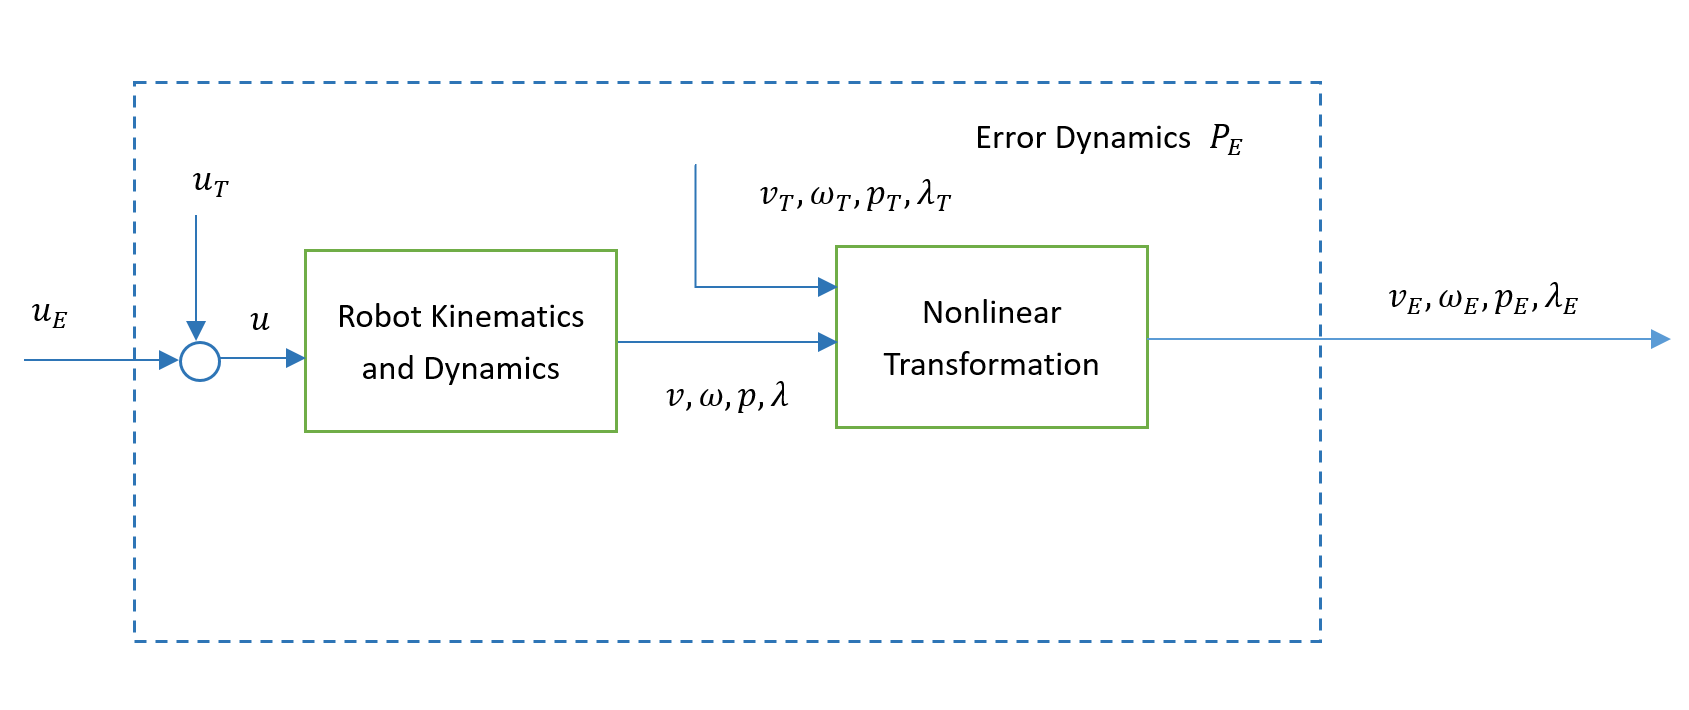
\includegraphics[width=0.9\textwidth]{NonlinearPlant.eps}
\caption{Nonliear transformation and error dynamics formulation}	
\label{FIG:NonlinearTransform}
\end{figure}
\section{Linearization of Error Dynamics}
\label{LinearizationMethods}
In the previous section, we have derived the error dynamic model for a given trim trajectory segment. In this section, we want to prove that the linearization for a specific trim trajectory segment $\vec{\eta}_{\mathcal{T}}$ is unique.

Firstly, we linearize the velocities error and get the following
equations:
\begin{empheq}[left=\empheqlbrace]{align}
&\dfrac{d}{dt}\delta\vec{v}_{E}=\emph{\textbf{A}}_{\vec{v}}^{\vec{v}}
\delta\vec{v}_{E}+\emph{\textbf{A}}_{\vec{v}}^{\vec{\omega}}
\delta\vec{\omega}_{E}+\emph{\textbf{A}}_{\vec{v}}^{\vec{\lambda}}
\delta\vec{\lambda}_{E}+\emph{\textbf{B}}_{\vec{v}}\delta\vec{u} \\
&\dfrac{d}{dt}\delta\vec{\omega}_{E}=\emph{\textbf{A}}_{\vec{\omega}}^{\vec{v}}
\delta\vec{v}_{E}+\emph{\textbf{A}}_{\vec{\omega}}^{\vec{\omega}}
\delta\vec{\omega}_{E}+\emph{\textbf{A}}_{\vec{\omega}}^{\vec{\lambda}}
\delta\vec{\lambda}_{E}+\emph{\textbf{B}}_{\vec{\omega}}\delta\vec{u} 
\end{empheq} 
where
\begin{empheq}[left=\empheqlbrace]{align}
&\emph{\textbf{A}}_{\vec{v}}^{\vec{v}}=\dfrac{\partial}{\partial \vec{v}}[\mathfrak{F}_{\vec{v}}(\vec{v},\vec{\omega})+\mathfrak{B}_{\vec{v}}(\vec{v},\vec{\omega})\mathfrak{H}(\vec{v},\vec{u})]
 \\
&\emph{\textbf{A}}_{\vec{v}}^{\vec{\omega}}=\dfrac{\partial}{\partial \vec{\omega}}[\mathfrak{F}_{v}(\vec{v},\vec{\omega})+\mathfrak{B}_{\vec{v}}(\vec{v},\vec{\omega})\mathfrak{H}(\vec{v},\vec{u})]
\\
&\emph{\textbf{A}}_{\vec{v}}^{\vec{\lambda}}=\dfrac{\partial}{\partial \vec{\lambda}}\mathfrak{F}_{\vec{v}}^{\vec{\lambda}}(\Pi_{i}\vec{\lambda})\\
&\emph{\textbf{B}}_{\vec{\upsilon}}=\dfrac{\partial}{\partial \vec{u}}
\mathfrak{B}_{\vec{v}}(\vec{v},\vec{\omega})\mathfrak{H}(\vec{v},\vec{u})
\end{empheq} 
and
\begin{empheq}[left=\empheqlbrace]{align}
&\emph{\textbf{A}}_{\vec{\omega}}^{\vec{v}}=\dfrac{\partial}{\partial \vec{v}}[\mathfrak{F}_{\omega}(\vec{v},\vec{\omega})+\mathfrak{B}_{\vec{\omega}}(\vec{v},\vec{\omega})\mathfrak{H}(\vec{v},\vec{u})]
 \\
&\emph{\textbf{A}}_{\vec{\omega}}^{\vec{\omega}}=\dfrac{\partial}{\partial \vec{\omega}}[\mathfrak{F}_{\omega}(\vec{v},\vec{\omega})+\mathfrak{B}_{\vec{\omega}}(\vec{v},\vec{\omega})\mathfrak{H}(\vec{v},\vec{u})]
\\
&\emph{\textbf{A}}_{\vec{\omega}}^{\vec{\lambda}}=\dfrac{\partial}{\partial \vec{\lambda}}\mathfrak{F}_{\vec{\omega}}^{\vec{\lambda}}(\Pi_{i}\vec{\lambda})\\
&\emph{\textbf{B}}_{\vec{\omega}}=\dfrac{\partial}{\partial \vec{u}}
\mathfrak{B}_{\vec{\omega}}(\vec{v},\vec{\omega})\mathfrak{H}(\vec{v},\vec{u}).
\end{empheq} 
Next, we want to show that the linearization of the position error $\vec{p}_{E}$ is time-invariant.
We define 
\begin{align}
\vec{f}_{\vec{p}_{E}}=\vec{v}
-\emph{\textbf{R}}_{E}^{-1}\vec{v}_{\mathcal{T}}
-\emph{\textbf{S}}(\vec{\omega}_{\mathcal{T}})\vec{p}_{E}
\end{align}
\begin{align}
\dfrac{d}{dt}\delta\vec{p}_{E}=
\underbrace{\dfrac{\partial \vec{f}_{\vec{p}_{E}}}{\partial \vec{v}_{E}}}_{(1)}\cdot\delta \vec{v}_{E}+
\underbrace{\dfrac{\partial \vec{f}_{\vec{p}_{E}}}{\partial \vec{\omega}_{E}}}_{(2)}\cdot\delta \vec{\omega}_{E}+
\underbrace{\dfrac{\partial \vec{f}_{\vec{p}_{E}}}{\partial \vec{p}_{E}}}_{(3)}\cdot\delta \vec{p}_{E}+
\underbrace{\dfrac{\partial \vec{f}_{\vec{p}_{E}}}{\partial \vec{\lambda}_{E}}}_{(4)}\cdot\delta \vec{\lambda}_{E}\label{EQ:PE1}
\end{align}
We calculate these four terms separately. 
Since $\vec{v}_{E}=\vec{v}-\vec{v}_{\mathcal{T}}$ and $\vec{v}_{\mathcal{T}}$ is a constant, we have
\begin{align}
(1):\dfrac{\partial \vec{f}_{\vec{p}_{E}}}{\partial \vec{v}_{E}}=\emph{\textbf{I}}_{3 \times 1}.\label{EQ:PE2}
\end{align}
\begin{align}
(2):\dfrac{\partial \vec{f}_{\vec{p}_{E}}}{\partial \vec{\omega}_{E}}=\emph{\textbf{0}}_{3 \times 1}.\label{EQ:PE3}
\end{align}
\begin{align}
(3):\dfrac{\partial \vec{f}_{\vec{p}_{E}}}{\partial \vec{p}_{E}}=
-\dfrac{\partial}{\partial \vec{p}_{E}}(\emph{\textbf{S}}(\vec{\omega}_{\mathcal{T}})\vec{p}_{E})\Bigr|_{\vec{\eta}=\vec{\eta}_{\mathcal{T}}}=-\emph{\textbf{S}}(\vec{\omega}_{\mathcal{T}}). \label{EQ:PE4}
\end{align}
\begin{align}
(4):\dfrac{\partial \vec{f}_{\vec{p}_{E}}}{\partial \vec{\lambda}_{E}}&=
-\dfrac{\partial}{\partial \vec{\lambda}}(\emph{\textbf{R}}_{E}^{-1}\vec{v}_{\mathcal{T}})
\dfrac{\partial \vec{\lambda}}{\partial \vec{\lambda}_{E}}\Bigr|_{\vec{\eta}=\vec{\eta}_{\mathcal{T}}} 
\nonumber \\
&=-\dfrac{\partial}{\partial \vec{\lambda}}(\emph{\textbf{R}}^{-1}\emph{\textbf{R}}_{\mathcal{T}}
\vec{v}_{\mathcal{T}})\dfrac{\partial \vec{\lambda}}{\partial \vec{\lambda}_{E}}\Bigr|_{\vec{\eta}=\vec{\eta}_{\mathcal{T}}} \nonumber \\
&=\emph{\textbf{S}}(\emph{\textbf{R}}^{-1}\emph{\textbf{R}}_{\mathcal{T}}\vec{v}_{\mathcal{T}})
\emph{\textbf{Q}}^{-1}
\dfrac{\partial \vec{\lambda}}{\partial \vec{\lambda}_{E}}\Bigr|_{\vec{\eta}=\vec{\eta}_{\mathcal{T}}} \label{EQ:FE1}
\end{align}
When the robot tracks the trim trajectory perfectly, we have the relationship:
\begin{align}
 \emph{\textbf{R}}_{\mathcal{T}}=\emph{\textbf{R}}. \label{EQ:FE2}
\end{align}
 Also we have
\begin{align}
\dfrac{\partial \vec{\lambda}}{\partial \vec{\lambda}_{E}}
=\dfrac{\partial (\emph{\textbf{Q}}\cdot\vec{\lambda}_{E}+\vec{\lambda}_{C})}{\partial \vec{\lambda}_{E}}
=\emph{\textbf{Q}}
\label{EQ:FE3}.
\end{align}
Combining \ref{EQ:FE1}, \ref{EQ:FE2} and \ref{EQ:FE3}, we obtain 
\begin{align}
(4):\dfrac{\partial \vec{f}_{\vec{p}_{E}}}{\partial \vec{\lambda}_{E}}=
\emph{\textbf{S}}(\vec{v}_{\mathcal{T}}).\label{EQ:PE5}
\end{align}
Taking \ref{EQ:PE2}, \ref{EQ:PE3}, \ref{EQ:PE4} and \ref{EQ:PE5} into \ref{EQ:PE1}, we obtain
\begin{align}
\dfrac{d}{dt}\delta\vec{p}_{E}=\delta \vec{v}_{E}-\emph{\textbf{S}}(\vec{\omega}_{\mathcal{T}})\delta \vec{p}_{E}-\emph{\textbf{S}}(\vec{v}_{\mathcal{T}})\delta\vec{\lambda}_{E}.
\end{align}
For the orientation dynamics, we linearize in the same way. We define
\begin{align}
\vec{f}_{\vec{\lambda}_{E}}=\vec{\omega}
-\emph{\textbf{Q}}^{-1}\emph{\textbf{Q}}_{\mathcal{T}}
\vec{\omega}_{\mathcal{T}}
+(\dfrac{d}{dt}\emph{\textbf{Q}}^{-1})\emph{\textbf{Q}}\vec{\lambda}_{E}
\end{align}
\begin{align}
\dfrac{d}{dt}\delta\vec{\lambda}_{E}=
\underbrace{\dfrac{\partial \vec{f}_{\vec{\lambda}_{E}}}{\partial \vec{v}_{E}}}_{(5)}\cdot\delta \vec{v}_{E}+
\underbrace{\dfrac{\partial \vec{f}_{\vec{\lambda}_{E}}}{\partial \vec{\omega}_{E}}}_{(6)}\cdot\delta \vec{\omega}_{E}+
\underbrace{\dfrac{\partial \vec{f}_{\vec{\lambda}_{E}}}{\partial \vec{p}_{E}}}_{(7)}\cdot\delta \vec{p}_{E}+
\underbrace{\dfrac{\partial \vec{f}_{\vec{\lambda}_{E}}}{\partial \vec{\lambda}_{E}}}_{(8)}\cdot\delta \vec{\lambda}_{E}\label{EQ:OE2}
\end{align}
$\vec{f}_{\vec{\lambda}_{E}}$ has nothing to do with $\vec{v}_{E}$ and $\vec{\omega}_{E}$, thus 
\begin{align}
(5): \dfrac{\partial \vec{f}_{\vec{\lambda}_{E}}}{\partial \vec{v}_{E}}=\vec{0}_{3\times 1},\label{EQ:OE3}
\end{align}
\begin{align}
(7): \dfrac{\partial \vec{f}_{\vec{\lambda}_{E}}}{\partial \vec{\lambda}_{E}}=\vec{0}_{3\times 1}.\label{EQ:OE4}
\end{align}
For angular velocity, we have
\begin{align}
(6): \dfrac{\partial \vec{f}_{\vec{\lambda}_{E}}}{\partial \vec{\omega}_{E}}=\dfrac{\partial\vec{\omega}}{\partial \vec{\omega}_{E}}=\dfrac{\partial (\vec{\omega}_{E}+\vec{\omega}_{\mathcal{T}})}{\partial \vec{\omega}}
=\emph{\textbf{I}}_{3 \times 3}.\label{EQ:OE5}
\end{align}
Along the trim trajectory $\vec{\eta}_{\mathcal{T}}$, the angular velocity transformation matrix $\emph{\textbf{Q}}^{-1}=\emph{\textbf{Q}}_{\mathcal{T}}^{-1}$, which is a constant matrix, thus 
\begin{align}
\dfrac{d}{dt}(\emph{\textbf{Q}}^{-1})\Bigr|_{\vec{\eta}=\vec{\eta}_{\mathcal{T}}}=\dfrac{d}{dt}(\emph{\textbf{Q}}_{\mathcal{T}}^{-1})=\vec{0}_{3\times 3}
\end{align}
and
\begin{align}
(\dfrac{d}{dt}\emph{\textbf{Q}}^{-1})\emph{\textbf{Q}}\vec{\lambda}_{E}\Bigr|_{\vec{\eta}=\vec{\eta}_{\mathcal{T}}}=\vec{0}_{3 \times 1}
\end{align}
Then, similar to the method for calculating the term (4)~\ref{EQ:FE1}, we have the following transformations:
\begin{align}
(8):\dfrac{\partial \vec{f}_{\vec{\lambda}_{E}}}{\partial \vec{\lambda}_{E}}
&=-\dfrac{\partial}{\partial \vec{\lambda}}(\emph{\textbf{Q}}^{-1}\emph{\textbf{Q}}_{\mathcal{T}}
\vec{\omega}_{\mathcal{T}})\dfrac{\partial \vec{\lambda}}{\partial \vec{\lambda}_{E}}\Bigr|_{\vec{\eta}=\vec{\eta}_{\mathcal{T}}} \nonumber \\
&=\emph{\textbf{S}}(\emph{\textbf{Q}}^{-1}\emph{\textbf{Q}}_{\mathcal{T}}\vec{\omega}_{\mathcal{T}})
\emph{\textbf{Q}}^{-1}
\dfrac{\partial \vec{\lambda}}{\partial \vec{\lambda}_{E}}\Bigr|_{\vec{\eta}=\vec{\eta}_{\mathcal{T}}} \nonumber \\
&=\emph{\textbf{S}}(\emph{\textbf{Q}}^{-1}\emph{\textbf{Q}}_{\mathcal{T}}\vec{\omega}_{\mathcal{T}})
\emph{\textbf{Q}}^{-1}\emph{\textbf{Q}}\Bigr|_{\vec{\eta}=\vec{\eta}_{\mathcal{T}}} \nonumber \\
&=\emph{\textbf{S}}(\emph{\textbf{Q}}^{-1}\emph{\textbf{Q}}_{\mathcal{T}}\vec{\omega}_{\mathcal{T}})
\Bigr|_{\vec{\eta}=\vec{\eta}_{\mathcal{T}}} \nonumber \\
&=\emph{\textbf{S}}(\vec{\omega}_{\mathcal{T}}).\label{EQ:OE6}
\end{align}
The orientation error dynamics can be summarized from~\ref{EQ:OE3}, \ref{EQ:OE4}, \ref{EQ:OE5}, \ref{EQ:OE6} as:
\begin{align}
\dfrac{d}{dt}\delta \vec{\lambda}_{E}=\delta\vec{\omega}_{E}-\emph{\textbf{S}}(\vec{\omega}_{\mathcal{T}})\delta \vec{\lambda}_{E}
\end{align}
To sum up, the linearized error dynamics is 
\begin{empheq}[left=\mathcal{P}_{E,L}:\empheqlbrace]{align}
&\dfrac{d}{dt}\delta\vec{x}_{dyn_{E}}=\emph{\textbf{A}}_{d}^{d}\delta\vec{x}_{dyn_{E}}+
\emph{\textbf{A}}_{k}^{d}\delta\vec{x}_{kin_{E}}+\emph{\textbf{B}}\vec{u} \\
&\dfrac{d}{dt}\delta\vec{x}_{kin_{E}}=\delta\vec{x}_{dyn_{E}}+\emph{\textbf{A}}_{k}^{k}
\delta\vec{x}_{kin_{E}}
\end{empheq}
where 
\begin{align}
\delta\vec{x}_{dyn_{E}}=
\begin{pmatrix}
\delta\vec{v}_{E}\\
\delta\vec{\omega}_{E}
\end{pmatrix}\in \mathbb{R}^{6}
\end{align} 
denotes the 6 dynamic error states (velocity errors) and
\begin{align}
\delta\vec{x}_{kin_{E}}=
\begin{pmatrix}
\delta \vec{p}_{E}\\
\delta \vec{\lambda}_{E}
\end{pmatrix} \in \mathbb{R}^{6}
\end{align}
The error dynamics system matrix $\emph{\textbf{A}}_{d}^{d}$ is defined as 
\begin{align}
\emph{\textbf{A}}_{d}^{d}=
\begin{pmatrix}
\emph{\textbf{A}}_{\vec{v}}^{\vec{v}}&\emph{\textbf{A}}_{\vec{v}}^{\vec{\omega}}\\
\emph{\textbf{A}}_{\vec{\omega}}^{\vec{v}}&\emph{\textbf{A}}_{\vec{\omega}}^{\vec{\omega}}
\end{pmatrix}\in \mathbb{R}^{6 \times 6}
\end{align}
indicating the mutual interaction between the linear velocities and angular velocities.
The error dynamics system matrix $\emph{\textbf{k}}_{d}^{d}$ is defined as
\begin{align}
\emph{\textbf{A}}_{k}^{d}=
\begin{pmatrix}
0&\emph{\textbf{A}}_{\vec{v}}^{\vec{\lambda}}\\
0&\emph{\textbf{A}}_{\vec{\omega}}^{\vec{\lambda}}
\end{pmatrix} \in \mathbb{R}^{6 \times 6}
\end{align}
representing the influence of the kinematic states on the dynamics states. It is noticeable that only the orientation states (Euler angles) 
$\vec{\lambda}_{E}$ have impact on the velocity errors $\vec{v}_{E}$ and 
$\vec{\omega}_{E}$. The robot dynamics is not dependent on its position. 
It can be identified from the robot dynamic equation~\ref{EQ:DecisionDynamics} and the restoring term definition~\ref{EQ:Restoring} that the robot dynamics is influenced by the roll angle $\phi$ and pitch angle $\theta$ due to the restoring part. 
The kinematic error system matrix $\emph{\textbf{A}}_{k}^{k}$ is defined as   
\begin{align}
\emph{\textbf{A}}_{k}^{k}=
\begin{pmatrix}
-\emph{\textbf{S}}(\vec{\omega}_{\mathcal{T}})&-\emph{\textbf{S}}(\vec{v}_{\mathcal{T}})\\
0&-\emph{\textbf{S}}(\vec{\omega}_{\mathcal{T}})
\end{pmatrix}\in \mathbb{R}^{6 \times 6},
\end{align}
The input matrix $\emph{\textbf{B}}$ is
\begin{align}
\emph{\textbf{B}}=
\begin{pmatrix}
\emph{\textbf{B}}_{\vec{v}}\\
\emph{\textbf{B}}_{\vec{\omega}}
\end{pmatrix} \in \mathbb{R}^{(n_{t}+n_{f})\times 6}.
\end{align}

From the previous analysis, we come to the conclusion that the linearized error dynamic system is a bijective function of trim trajectories $\vec{\eta}_{\mathcal{T}}=(||\vec{v}_{\mathcal{T}}||,   \dot{\psi}_{\mathcal{T}}, \gamma_{\mathcal{T}})^{T}$. This property is of significance since we can adopt the methods for MIMO linear systems to handle the originally nonlinear and strongly coupled system. 

A system is said to be controllable at time $t_{0}$ if the system can be transferred from any initial state $\vec{x}(t_{0})$ to any other state in a finite interval of time by means of an unconstrained control input. 
For the actuator optimization problem in the next chapter, the controllability is the primal requirement of a certain actuator configuration. The error dynamics is completely state controllable if and only if the vectors $\textbf{\emph{B}}_{E}$, $\textbf{\emph{A}}_{E}\textbf{\emph{B}}_{E}$, \ldots, $\textbf{\emph{A}}_{E}^{11}\textbf{\emph{B}}_{E}$ are linearly independent, which can be also checked with the controllability matrix which is defined as
\begin{align}
\emph{\textbf{C}}=[\textbf{\emph{B}}_{E} \quad \textbf{\emph{A}}_{E}\textbf{\emph{B}}_{E} \quad \ldots \quad \textbf{\emph{A}}_{E}^{11}\textbf{\emph{B}}_{E}].
\end{align}
An LTI system is controllable if the controllability matrix $\mathcal{C}$ has full row rank. In our case, we expect the rank of the controllability matrices all trim trajectory segments to be equal to 12. That is 
\begin{align}
rank(\emph{\textbf{C}}_{E,1})&=12 \nonumber \\
& \vdots \nonumber \\
rank(\emph{\textbf{C}}_{E,m})&=12
\end{align}
\section{Switched LQR Controller Design for Trim Trajectories}
In the previous two sections, we have proved that the linearized error dynamics is unique for each trim trajectory segment. For the whole trajectory consisting of a group of trim trajectores, the error dynamics can be formulated as a switched system.   
Suppose we have $m$ linearized trim trajectory error dynamics,
\begin{align}
\dot{\vec{x}}_{E,1} &=\emph{\textbf{A}}_{E,1}\vec{x}_{E,1}+\emph{\textbf{B}}_{E,1}
\vec{u}_{E,1} \nonumber \\
\dot{\vec{x}}_{E,2} &=\emph{\textbf{A}}_{E,2}\vec{x}_{E,2} +\emph{\textbf{B}}_{E,2}
\vec{u}_{E,2}\nonumber \\
& \vdots \nonumber \\
\dot{\vec{x}}_{E,m} &=\emph{\textbf{A}}_{E,m}\vec{x}_{E,m}+\emph{\textbf{B}}_{E,m}
\vec{u}_{E,m},
\end{align}
where $\vec{x}_{E,1}=(\vec{v}_{E,1}, \vec{\omega}_{E,1}, \vec{p}_{E,1}, \vec{\lambda}_{E,1})^{T}, \cdots, \vec{x}_{E,m}=(\vec{p}_{E,m}, \vec{\lambda}_{E,m}, \vec{v}_{E,m}, \vec{\omega}_{E,m})^{T}$ are error states using the nonlinear transformations \ref{EQ:NLT1}, \ref{EQ:NLT2}, \ref{EQ:NLT3} and \ref{EQ:NLT4}. The error dynamics system matrix $\emph{\textbf{A}}_{E,j}, j=1, \cdots, m$ is 
\begin{align}
\emph{\textbf{A}}_{E,j}=
\begin{pmatrix}
&\emph{\textbf{A}}_{d,j}^{d}&\emph{\textbf{A}}_{k,j}^{d} \\
&\emph{\textbf{I}}_{3\times3}&\emph{\textbf{A}}_{d,j}^{d}
\end{pmatrix} \in \mathbb{R}^{12\times 12}
\end{align}
and the error dynamics input matrix $\emph{\textbf{B}}_{E,j}$ is
\begin{align}
\emph{\textbf{B}}_{E,j}=
\begin{pmatrix}
\emph{\textbf{B}}_{\vec{v},j} \\
\emph{\textbf{B}}_{\vec{\omega},j}
\end{pmatrix} \in \mathbb{R}^{12\times (p+q)}.
\end{align}
Both of them are calculated with linearization methods in Section~\ref{LinearizationMethods}. 

For each trim trajectory segment, we have a 12-dimensional MIMO linear system, thus we design a LQR controller with weighting matrix $ \mathcal{Q}_{E,j} $ and $\mathcal{R}_{E,j}$ to minimize the cost function for the j-th trim trajectory
\begin{align}
J=\int^{\infty}_{0}[\vec{x}_{E,j}^{T}\mathcal{Q}_{E,j}\vec{x}_{E,j}+\vec{u}_{E,j}^{T}\mathcal{R}_{E,j}
\vec{u}_{E,j}]dt
\end{align}
subject to $\vec{x}_{E,j}(0)=\vec{x}_{E,j,0}$, $\mathcal{Q}_{E,j} \succeq 0$, $\mathcal{Q}_{E,j}^{T}=\mathcal{Q}_{E,j}$, $\mathcal{R}_{E,j} \succ 0$ and $\mathcal{R}_{E,j}^{T}=\mathcal{R}_{E,j}$.
Assume that ($\emph{\textbf{A}}_{E,j}$,~$\emph{\textbf{B}}_{E,j}$) is controllable, the optimal solution to minimize the cost function is $\vec{u}_{E,j}=-\mathcal{K}_{j}\vec{x}_{E,j}$,
where $\mathcal{K}_{j}=\mathcal{R}_{E,j}^{-1}\emph{\textbf{B}}_{E,j}^{T}
\emph{\textbf{S}}_{E,j}$ is a constant linear state feedbak gain.

The matrix $\emph{\textbf{S}}_{E}\succeq 0$  which is the solution of the continuous Algebraic Riccati Equation (ARE):

\begin{align}
\mathcal{Q}_{E,j}+\emph{\textbf{A}}_{E,j}^{T}\emph{\textbf{S}}_{E,j}
+\emph{\textbf{S}}_{E,j}\emph{\textbf{A}}_{E,j}
-\emph{\textbf{S}}_{E,j}\emph{\textbf{B}}_{E,j}\mathcal{R}_{E,j}^{-1}
\emph{\textbf{B}}_{E,j}^{T}\emph{\textbf{S}}_{E,j}=0.
\end{align}

\section{Stability-based Selection of Weighting Matrices}

After we implement the state feedback $\vec{u}_{E,j}=-\mathcal{K}_{j}\vec{x}_{E,j}$ to the error dynamics system $\dot{\vec{x}}_{E,j} =\emph{\textbf{A}}_{E,j}\vec{x}_{E,j}+\emph{\textbf{B}}_{E,j}
\vec{u}_{E,j}$ for the j-th trim trajectory, we obtain the closed loop error dynamics system:
\begin{align}
\dot{\vec{x}}_{E,j}=\emph{\textbf{A}}_{E,j}\vec{x}_{E,j}
+\emph{\textbf{B}}_{E,j}\vec{u}_{E,j} \nonumber \\
=(\emph{\textbf{A}}_{E,j}
-\emph{\textbf{B}}_{E,j}\mathcal{K}_{j})\cdot \vec{x}_{E,j}
\end{align}

We want prove that each trim trajectory can be stabilized by the corresponding LQR controller.
Define the Lyapunov function $V_{E,j}(\vec{x}_{E,j})
=\vec{x}_{E,j}^{T}\emph{\textbf{S}}_{E,j}\vec{x}_{E,j}, j=1, \cdots, m$, where $\emph{\textbf{S}}_{E}$ is positive definite and symmetric, $\emph{\textbf{S}}_{E}\succeq 0,~\emph{\textbf{S}}_{E}^{T}=\emph{\textbf{S}}_{E}$.  Differentiating it we obtain 
\begin{align}
\dot{V}_{E,j}(\vec{x}_{E,j})&=
\dot{\vec{x}}_{E,j}^{T}\emph{\textbf{S}}_{E,j}\vec{x}_{E,j}+
\vec{x}_{E,j}^{T}\emph{\textbf{S}}_{E,j}\dot{\vec{x}}_{E,j} \nonumber \\
&= \left[(\emph{\textbf{A}}_{E,j}-
\emph{\textbf{B}}_{E,j}\mathcal{K}_{E,j})\vec{x}_{E,j}\right]^{T}
\emph{\textbf{S}}_{E,j}\vec{x}_{E,j}+\vec{x}_{E,j}^{T}\emph{\textbf{S}}_{E,j}
[(\emph{\textbf{A}}_{E,j}-\emph{\textbf{B}}_{E,j}\mathcal{K}_{E,j})\vec{x}_{E,j}]
\nonumber \\
\overset{\mathcal{K}_{E,j}
=\mathcal{R}_{E}^{-1}\emph{\textbf{B}}_{E,j}^{T}\emph{\textbf{S}}_{E,j}}{=}
&\vec{x}_{E,j}^{T}\left[\underbrace{(\emph{\textbf{A}}_{E,j}-
\emph{\textbf{B}}_{E,j}\mathcal{R}_{E,j}^{-1}\emph{\textbf{B}}_{E,j}^{T}
\emph{\textbf{S}}_{E,j})^{T}\emph{\textbf{S}}_{E,j}}_{(1)}
+
\underbrace{\emph{\textbf{S}}_{E,j}
(\emph{\textbf{A}}_{E,j}-\emph{\textbf{B}}_{E,j}
\mathcal{R}_{E,j}^{-1}\emph{\textbf{B}}_{E,j}^{T}\emph{\textbf{S}}_{E,j})}_{(2)}
\right]
\vec{x}_{E,j}
\end{align}
\begin{align}
(1)=(\emph{\textbf{A}}_{E,j}^{T}-\emph{\textbf{S}}_{E,j}^{T}
\emph{\textbf{B}}_{E,j}(\mathcal{R}_{E,j}^{-1})^{T}
\emph{\textbf{B}}_{E,j}^{T})\emph{\textbf{S}}_{E,j} \nonumber \\
=(\emph{\textbf{A}}_{E,j}^{T}
-\emph{\textbf{S}}_{E,j}\emph{\textbf{B}}_{E,j}\mathcal{R}^{-1}_{E,j}
\emph{\textbf{B}}^{T}_{E,j})\emph{\textbf{S}}_{E,j} \nonumber \\
=\emph{\textbf{A}}_{E,j}^{T}\emph{\textbf{S}}_{E,j}
-\emph{\textbf{S}}_{E,j}\emph{\textbf{B}}_{E,j}\mathcal{R}^{-1}_{E,j}
\emph{\textbf{B}}^{T}_{E,j}\emph{\textbf{S}}_{E,j}
\end{align}
\begin{align}
(2)=\emph{\textbf{S}}_{E,j}\emph{\textbf{A}}_{E,j}-\emph{\textbf{S}}_{E,j}
\emph{\textbf{B}}_{E,j}\mathcal{R}^{-1}_{E,j}
\emph{\textbf{B}}^{T}_{E,j}\emph{\textbf{S}}_{E,j} \nonumber \\
=\emph{\textbf{S}}_{E,j}\emph{\textbf{A}}_{E,j}-\emph{\textbf{S}}_{E,j}^{T}
\emph{\textbf{B}}_{E,j}\mathcal{R}^{-1}_{E,j}
\emph{\textbf{B}}^{T}_{E,j}\emph{\textbf{S}}_{E,j}
\end{align}
\begin{align}
(1)+(2)=\emph{\textbf{A}}_{E,j}^{T}\emph{\textbf{S}}_{E,j}
-\emph{\textbf{S}}_{E,j}\emph{\textbf{B}}_{E,j}\mathcal{R}^{-1}_{E,j}
\emph{\textbf{B}}^{T}_{E,j}\emph{\textbf{S}}_{E,j}+
\emph{\textbf{S}}_{E,j}\emph{\textbf{A}}_{E,j}-\emph{\textbf{S}}_{E,j}^{T}
\emph{\textbf{B}}_{E,j}\mathcal{R}^{-1}_{E,j}
\emph{\textbf{B}}^{T}_{E,j}\emph{\textbf{S}}_{E,j} \nonumber \\
\overset{ARE}{=}
-\mathcal{Q}_{E,j}-\emph{\textbf{S}}_{E,j}^{T}\emph{\textbf{B}}_{E,j}
\mathcal{R}^{-1}_{E,j}
\emph{\textbf{B}}^{T}_{E,j}\emph{\textbf{S}}_{E,j}
\end{align}
Since $\mathcal{R}_{E,j}$ is diagonal and positive definite, its inverse is also diagonal and positive definite, i.e., $\mathcal{R}_{E,j}\succ 0\Rightarrow \mathcal{R}_{E,j}^{-1} \succ 0$, then $\emph{\textbf{S}}_{E,j}^{T}\emph{\textbf{B}}_{E,j}
\mathcal{R}^{-1}_{E,j}
\emph{\textbf{B}}^{T}_{E,j}\emph{\textbf{S}}_{E,j} \succ 0$, since $\mathcal{Q}_{E,j} \succeq 0$, we have $\dot{V}_{E,j}(\vec{x}_{E,j})=(1)+(2) \prec 0$. The derivative of the Lyapunov function is negative definite, so the error dynamics system can be asymptotically stabilized by the LQR state feedback controller $\vec{u}_{E,j}=-\mathcal{K}\vec{x}_{E,j}$ at the equilibrium point $\vec{x}_{E,j}=0$. Note that the error dynamics input $\vec{u}_{E,j}=\vec{u}_{j}-\vec{u}_{\mathcal{T}_{j}}$, then the input $\vec{u}_{j}$ given into the nonlinear underwater dynamic system for the j-th trim trajectory is 
\begin{align}
\vec{u}_{j}=\vec{u}_{E,j}+\vec{u}_{\mathcal{T}_{j}} \nonumber \\
=\vec{u}_{\mathcal{T}_{j}}-\mathcal{K}\vec{x}_{E,j},
\end{align} 
where $\vec{u}_{\mathcal{T}_{j}}$ is the constant desired trim input for the j-th trim trajectory segment. The input $\vec{u}_{j}$ is composed of a constant feedforward input $\vec{u}_{\mathcal{T}_{j}}$ and a state feedback $-\mathcal{K}\vec{x}_{E,j}$.

When we implement all the corresponding LQR state feedback controller to all trim trajectory segments, we obtain
\begin{align}
\dot{\vec{x}}_{E,1} &=(\emph{\textbf{A}}_{E,1}-
\mathcal{R}_{E,1}\emph{\textbf{B}}^{T}_{E,1}
\emph{\textbf{S}}_{E,1})\vec{x}_{E,1} \nonumber \\
\dot{\vec{x}}_{E,2} &=(\emph{\textbf{A}}_{E,2}-
\mathcal{R}_{E,2}\emph{\textbf{B}}^{T}_{E,2}
\emph{\textbf{S}}_{E,2})\vec{x}_{E,2} \nonumber \\
& \vdots \nonumber \\
\dot{\vec{x}}_{E,m} &=(\emph{\textbf{A}}_{E,m}-
\mathcal{R}_{E,m}\emph{\textbf{B}}^{T}_{E,m}
\emph{\textbf{S}}_{E,m})\vec{x}_{E,m}
\end{align}
If we denote the closed system matrix as
\begin{align}
\bar{\emph{\textbf{A}}}_{E,1}&=\emph{\textbf{A}}_{E,1}-
\mathcal{R}_{E,1}\emph{\textbf{B}}^{T}_{E,1}
\emph{\textbf{S}}_{E,1} \nonumber \\
\bar{\emph{\textbf{A}}}_{E,2}&=\emph{\textbf{A}}_{E,2}-
\mathcal{R}_{E,2}\emph{\textbf{B}}^{T}_{E,2}
\emph{\textbf{S}}_{E,2} \nonumber \\
& \vdots \nonumber \\
\bar{\emph{\textbf{A}}}_{E,m}&=\emph{\textbf{A}}_{E,m}-
\mathcal{R}_{E,m}\emph{\textbf{B}}^{T}_{E,m}
\emph{\textbf{S}}_{E,m}
\end{align}
Then we can represent the closed loop error dynamics as
follows:
\begin{align}
\dot{\vec{x}}_{E,1}&=\bar{\emph{\textbf{A}}}_{E,1}\vec{x}_{E,1} \nonumber \\
\dot{\vec{x}}_{E,2}&=\bar{\emph{\textbf{A}}}_{E,2}\vec{x}_{E,2}
 \nonumber 
\\
\vdots \nonumber \\
\dot{\vec{x}}_{E,m}&=\bar{\emph{\textbf{A}}}_{E,m}\vec{x}_{E,m}
\end{align}
Thus, we can define our closed-loop error dynamics as a switched system 
\begin{align}
\Sigma_{S,\bar{\emph{\textbf{A}}}_{E}}: \dot{\vec{x}}_{E}(t)=
\bar{\emph{\textbf{A}}}_{E}(t)\vec{x}_{E}(t)
\end{align}
where $\bar{\emph{\textbf{A}}}_{E}(t)\in\lbrace \bar{\emph{\textbf{A}}}_{E,1},\ldots,\bar{\emph{\textbf{A}}}_{E,m}\rbrace$.


LQR controller can ensure the stability of each trim trajectory segment, however it can not ensure the stability of the whole trajectory. The stability for arbitrary switching can be proven by means of common quadratic lyapunov functions~(CQLFs) (\cite{Shorten2007}). Recall that $V_{E,j}(\vec{x}_{E,j})=\vec{x}_{E,j}^{T}\emph{\textbf{S}}_{E,j}\vec{x}_{E,j}$ is a quadratic Lyapunov function (QLF) for the LTI system: $\vec{x}_{E,j}=\bar{\emph{\textbf{A}}}_{E,j}(t)\vec{x}_{E,j}(t)$, where $\emph{\textbf{S}}_{E,j}$ is symmetric and positive definite satisfying $\emph{\textbf{S}}_{E,j}\bar{\emph{\textbf{A}}}_{E,j}
+\bar{\emph{\textbf{A}}}_{E,j}^{T}\emph{\textbf{S}}_{E,j}$ is negative definite. The existence of CQLF $V(\vec{x}_{E})=\vec{x}_{E}^{T}\emph{\textbf{S}}_{E}\vec{x}_{E}$ is equivalent to determine whether such a matrix $\emph{\textbf{S}}_{E}$ exists for a given group of Hurwitz matrices $\left\lbrace\emph{\textbf{A}}_{E,1}, \emph{\textbf{A}}_{E,2}, \ldots,\emph{\textbf{A}}_{E,m}\right\rbrace$ such that
\begin{align}
\bar{\emph{\textbf{A}}}_{E,1}^{T}\emph{\textbf{S}}_{E}
+\emph{\textbf{S}}_{E}\bar{\emph{\textbf{A}}}_{E,1} &\prec 0 \nonumber \\
\bar{\emph{\textbf{A}}}_{E,2}^{T}\emph{\textbf{S}}_{E}
+\emph{\textbf{S}}_{E}\bar{\emph{\textbf{A}}}_{E,1} &\prec 0 \nonumber \\
& \vdots \nonumber \\
\bar{\emph{\textbf{A}}}_{E,m}^{T}\emph{\textbf{S}}_{E}
+\emph{\textbf{S}}_{E}\bar{\emph{\textbf{A}}}_{E,m} & \prec 0,\label{EQ:LMI0}
\end{align} 
This is a system of linear matrix inequalities (LMIs), it is said to be feasible if a solution $\emph{\textbf{S}}_{E}$ exists. Otherwise, the LMIs are infeasible. 
Thus, determining whether or not the switched system $\Sigma_{S,\bar{\emph{\textbf{A}}}_{E}}$ has a CQLF amounts to checking the feasibility of a system of LMIs~\cite{Shorten2007}. 
Converting these to the nonstrict LMIs 
\begin{align}
\bar{\emph{\textbf{A}}}_{E,1}^{T}\emph{\textbf{S}}_{E}
+\emph{\textbf{S}}_{E}\bar{\emph{\textbf{A}}}_{E,1} &\preceq \emph{\textbf{I}} \nonumber \\
\bar{\emph{\textbf{A}}}_{E,2}^{T}\emph{\textbf{S}}_{E}
+\emph{\textbf{S}}_{E}\bar{\emph{\textbf{A}}}_{E,2} &\preceq 
\emph{\textbf{I}} \nonumber \\
& \vdots \nonumber \\
\bar{\emph{\textbf{A}}}_{E,m}^{T}\emph{\textbf{S}}_{E}
+\emph{\textbf{S}}_{E}\bar{\emph{\textbf{A}}}_{E,m} & \preceq \emph{\textbf{I}}
\label{EQ:LMI1}
\end{align} 
\begin{align}
\emph{\textbf{S}}_{E} \succeq \emph{\textbf{I}}. \label{EQ:LMI2}
\end{align}
This can be formulated as semidefinite programming so that we can utilize the CVX~\cite{cvx,gb08} to check whether a matrix $\emph{\textbf{S}}_{E}$ satisfying the aforementioned LMIs can be found. 

Recall that $\bar{\emph{\textbf{A}}}_{E,j}, j=1, \cdots, m$ is the closed loop system matrix after we implement the state feedback gain, $\vec{u}_{E}=-\mathcal{R}_{E}^{-1}\emph{\textbf{B}}_{E,j}\emph{\textbf{S}}_{E}$
where specified weighting matrices $\mathcal{Q}_{E,j}$ and $\mathcal{R}_{E,j}$ are user-defined and $\emph{\textbf{S}}_{E}$ is calulated from AREs. The LMIs~\ref{EQ:LMI0} can be rewritten as:
\begin{align}
(\emph{\textbf{A}}_{E,1}-
\mathcal{R}_{E,1}\emph{\textbf{B}}^{T}_{E,1}
\emph{\textbf{S}}_{E})^{T}\emph{\textbf{S}}_{E}
+\emph{\textbf{S}}_{E}(\emph{\textbf{A}}_{E,1}-
\mathcal{R}_{E,1}\emph{\textbf{B}}^{T}_{E,1}
\emph{\textbf{S}}_{E}) &\prec 0 \nonumber \\
(\emph{\textbf{A}}_{E,2}-
\mathcal{R}_{E,2}\emph{\textbf{B}}^{T}_{E,2}
\emph{\textbf{S}}_{E})^{T}\emph{\textbf{S}}_{E}
+\emph{\textbf{S}}_{E}(\emph{\textbf{A}}_{E,2}-
\mathcal{R}_{E,2}\emph{\textbf{B}}^{T}_{E,1}
\emph{\textbf{S}}_{E}) &\prec 0 \nonumber \\
& \vdots \nonumber \\
(\emph{\textbf{A}}_{E,m}-
\mathcal{R}_{E,m}\emph{\textbf{B}}^{T}_{E,m}
\emph{\textbf{S}}_{E})^{T}\emph{\textbf{S}}_{E}
+\emph{\textbf{S}}_{E}(\emph{\textbf{A}}_{E,m}-
\mathcal{R}_{E,m}\emph{\textbf{B}}^{T}_{E,m}
\emph{\textbf{S}}_{E}) & \prec 0.
\label{EQ:LMI4}
\end{align} 
Besides, the existence of a common $\emph{\textbf{S}}_{E}$ means all AREs of all trim trajectories possess the same solution:
\begin{align}
\mathcal{Q}_{E,1}+\emph{\textbf{A}}_{E,1}^{T}\emph{\textbf{S}}_{E}
+\emph{\textbf{S}}_{E}\emph{\textbf{A}}_{E,1}
-\emph{\textbf{S}}_{E}\emph{\textbf{B}}_{E,1}\mathcal{R}_{E,1}^{-1}
\emph{\textbf{B}}_{E}^{T}\emph{\textbf{S}}_{E}=0 \nonumber \\
\vdots \nonumber \\
\mathcal{Q}_{E,m}+\emph{\textbf{A}}_{E,m}^{T}\emph{\textbf{S}}_{E}
+\emph{\textbf{S}}_{E}\emph{\textbf{A}}_{E,m}
-\emph{\textbf{S}}_{E}\emph{\textbf{B}}_{E,m}\mathcal{R}_{E,m}^{-1}
\emph{\textbf{B}}_{E}^{T}\emph{\textbf{S}}_{E}=0\label{EQ:LMI5}
\end{align} 

Thus, there are coupling between the selections of the weighting matrices $\mathcal{Q}_{E,1}, \cdots, \mathcal{Q}_{E,m}$ and $\mathcal{R}_{E,1}, \cdots, \mathcal{R}_{E,m}$ and their values play an essential role for the global stability of the switched system.

Thus, the first step to design the switched LQR controller is to select the values of $\mathcal{R}_{E,1}, \cdots, \mathcal{R}_{E,m}$. Because tracking the specified trajectories is the most significant, the weighting coefficients for positions should be bigger than those of the Euler angles and velocities weighting coefficients should be smaller than both of them. Then, using $m$ state costing matrices we could solve the LMIs~\ref{EQ:LMI4} to find a common matrix $\emph{\textbf{S}}_{E}$. With the values of $\mathcal{R}_{E,1}, \cdots, \mathcal{R}_{E,m}$ and the matrix $\emph{\textbf{S}}_{E}$, the another corresponding weighting matrix $\mathcal{Q}_{E,j}, j=1, \cdots, m$ penalizing the error states $\vec{x}_{E,j}$ can be calculated from the corresponding ARE~\ref{EQ:LMI5}.  



